%\section{Results}

In this section, we present our experimental results on {\em E. coli} and GenomeTrakr data. We show the scalability of $\ours$ by demonstrating the time and computational resources needed to build the colored de Bruijn graph for 16,000 strains of salmonella.  Next, in order to validate the correctness of our approach, we generated two succinct colored de Bruijn graphs with sets of three  \emph{E. coli} assemblies each, merged them, and verified its equivalence to a six color graph built from scratch.  This experiment demonstrates that the merged colored de Bruijn graph is equivalent to that produced by building the graph without merging.    We ran all performance experiments on a machine with two Xeon E5-2640 v4 chips, each having 10 2.4 GHz cores.  The system contains 755 GB of RAM and two ZFS RAID pools of 9 disk each for storage.  We report wall clock time and maximum resident set size from Linux.  We use the SDSL-Lite library~\cite{SDSL} to store all succinct vectors. %We report all time in CPU time.
 

%%%%%%%%%%%%%%%%%%%%%%%%%%%%%%%%%%%%%%%%%%%%%%%%%%%%%%%%%%%%%%%%%%%%%%%%%%%%%%%%%%%%%%%%%%%%%%%%%%%%%%%%%%%%%%%%%%%%%%%%%%%%%%%%%

\begin{table*}[t]
\footnotesize
\begin{center}
%\vspace{8mm}
%{\setlength{\tabcolsep}{1em}
\begin{tabular}{|l|r|r|r|r|r|r|r|r|r|r|r|r|}
  \hline
  &  \multicolumn{2}{|c|}{Input Stats} & \multicolumn{3}{|c|}{de Bruijn Graph } & \multicolumn{3}{|c|}{Color Matrix } & \multicolumn{4}{|c|}{Combined Requirements}\\
  \hline

\textbf{Program and Dataset} & \textbf{$k$-mers} & \textbf{Colors} & \textbf{ RAM}& \textbf{Time} & \textbf{Size} & \textbf{RAM} &   \textbf{Time} & \textbf{Size} &  \textbf{RAM}  & \textbf{Ext. Mem.}  &   \textbf{Time} & \textbf{Size} \\ 
\hline

$\vari$(8k-1)   & 2.4 B       & 8,000 &              271 GB      & 30 h 49 m & 0.63 GB &              117 GB     & 6 h 28 m   & 114 GB              &    271 GB  & 4.6 TB  & 37 h  27 m &  114 GB \\
$\ours$(8k-1)      & 2.4 B     & 8,000 &              137 GB      & 21 h 27 m & 0.63 GB &              117 GB    & 5 h 3 m    & 114 GB               &    137 GB  & 1.5 TB  & 26 h  30 m & 114 GB\\


%$\vari$-C(8k-1) & 2.4 B    & 8,000 & 117 GB & N/A     & 6 h 28 m & 106 GB \\

\hline

\hline
\end{tabular}
\label{tab:compare}
\caption{Comparison between building a succinct colored de Bruijn for the same 8,000 Salmonella strains using $\vari$ versus $\ours$.}
%\caption{Performance statistics for $\vari$ and $\ours$. We separately list the succinct de Bruijn graph producing programs (labeled $\vari$ and $\ours$) from the color annotation matrix producing programs (labeled $\vari$-C and $\ours$-C). The total size of a succinct colored de Bruijn graph is comprised of the space for the succinct de Bruijn graph plus the space for the color matrix. }
\end{center}
\end{table*}
%%%%%%%%%%%%%%%%%%%%%%%%%%%%%%%%%%%%%%%%%%%%%%%%%%%%%%%%%%%%%%%%%%%%%%%%%%%%%%%%%%%%%%%%%%%%%%%%%%%%%%%%%%%%%%%%%%%%%%%%%%%%%%%%%

%%%%%%%%%%%%%%%%%%%%%%%%%%%%%%%%%%%%%%%%%%%%%%%%%%%%%%%%%%%%%%%%%%%%%%%%%%%%%%%%%%%%%%%%%%%%%%%%%%%%%%%%%%%%%%%%%%%%%%%%%%%%%%%%%
\begin{table*}[t]
\footnotesize
\begin{center}
%\vspace{8mm}
%{\setlength{\tabcolsep}{1em}
\begin{tabular}{|r|r|r|r|r|r|r|r|r|r|r|r|r|}
  \hline
  &  \multicolumn{2}{|c|}{Input Stats} & \multicolumn{3}{|c|}{de Bruijn Graph } & \multicolumn{3}{|c|}{Color Matrix } & \multicolumn{4}{|c|}{Combined Requirements}\\
  \hline

\textbf{Program and Dataset} & \textbf{$k$-mers} & \textbf{Colors} & \textbf{ RAM}& \textbf{Time} & \textbf{Size} & \textbf{RAM} &   \textbf{Time} & \textbf{Size} &  \textbf{RAM}  & \textbf{Ext. Mem.}  &   \textbf{Time} & \textbf{Size} \\ 
\hline
$\vari$(4k-1)      & 1.1 B    & 4,000 &               136 GB      & 8 h 46 m  & 0.31 GB &              52 GB     & 1 h 39 m & 51.2 GB               & 136 GB & 1 TB    & 10 h 25 m & 51 GB \\
$\vari$(4k-2)      & 1.5 B    & 4,000 &              137 GB      & 10 h 40 m & 0.52 GB &              54 GB     & 2 h 22 m & 52.5 GB                &  137 GB & 1.5 TB  &  13 h  2 m & 53 GB\\
$\merge$(4k-1, 4k-2)  & 2.4 B    & 8,000 &              10 GB       & 2 h 1 m   & 0.63 GB &              117 GB    & 1 h  2 m & 106 GB               &  117 GB    &  N/A    &  3 h 3 m & 106 GB \\

\hline
$\ours$(8k-1)      & 2.4      & 8,000 &              137 GB      & 21 h 27 m & 0.63 GB &              117 GB    & 5 h 3 m  & 117 GB               &    137 GB  & 1.5 TB  & 26 h  30 m & 106 GB\\

%$\vari$-C(4k-1) & 1.1 B    & 4,000 & 52 GB  & N/A     & 1 h 39 m & 51.2 GB \\
%$\vari$-C(4k-2) & 1.5 B    & 4,000 & 54 GB  & N/A     & 2 h 22 m & 52.5 GB \\
%$\ours$-C(4k-1, 4k-2)  & 2.4 B & 8,000 & 117 GB & N/A & 1 h 2 m & 106 GB \\
\hline



\hline
\end{tabular}
\label{tab:breakdown}
\caption{Breakdown of the components of $\ours$ which was listed in Table 1. The $\ours$ method consists of running $\vari$ on subsets of the population (4k-1 and 4k-2) and then merging the results with our proposed merge algorithm (denoted merge here).  Here we list the resources used for both individual runs of VARI as well as the merge.  We also list the combined resources, consisting of the total time and maximum space used across all three components of $\ours$ used in this dataset. Both $\vari$ and our merge algorithm each consist of two programs: one primarily responsible for the succinct de Bruijn graph and one for compressing the color matrix.  The resources for these are listed in separate columns and the combined resources needed for each method in the rightmost columns.  Size is the resulting succinct data structure size.}
%\caption{Performance statistics for $\vari$ and $\ours$. We separately list the succinct de Bruijn graph producing programs (labeled $\vari$ and $\ours$) from the color annotation matrix producing programs (labeled $\vari$-C and $\ours$-C). The total size of a succinct colored de Bruijn graph is comprised of the space for the succinct de Bruijn graph plus the space for the color matrix. }
\end{center}
\end{table*}
%%%%%%%%%%%%%%%%%%%%%%%%%%%%%%%%%%%%%%%%%%%%%%%%%%%%%%%%%%%%%%%%%%%%%%%%%%%%%%%%%%%%%%%%%%%%%%%%%%%%%%%%%%%%%%%%%%%%%%%%%%%%%%%%%



%%%%%%%%%%%%%%%%%%%%%%%%%%%%%%%%%%%%%%%%%%%%%%%%%%%%%%%%%%%%%%%%%%%%%%%%%%%%%%%%%%%%%%%%%%%%%%%%%%%%%%%%%%%%%%%%%%%%%%%%%%%%%%%%%
\begin{table*}[h!]
\footnotesize
\begin{center}
%\vspace{8mm}
%{\setlength{\tabcolsep}{1em}
\begin{tabular}{|l|r|r|r|r|r|r|r|r|r|r|r|r|}
  \hline
  &  \multicolumn{2}{|c|}{Input Stats} & \multicolumn{3}{|c|}{de Bruijn Graph} & \multicolumn{3}{|c|}{Color Matrix} & \multicolumn{4}{|c|}{Combined Requirements}\\
  \hline

\textbf{Program and Dataset} & \textbf{$k$-mers} & \textbf{Colors} & \textbf{ RAM}& \textbf{Time} & \textbf{Size} & \textbf{RAM} &   \textbf{Time} & \textbf{Size} &  \textbf{RAM}  & \textbf{Ext. Mem.}  &   \textbf{Time} & \textbf{Size} \\ 
\hline

%$\vari$(4k-1)      & 1.1 B    & 4,000 &               136 GB      & 8 h 46 m  & 0.31 GB &              52 GB     & 1 h 39 m & 51.2 GB               & 136 GB & 1 TB    & 10 h 25 m & 51 GB \\
$\vari$(4k-3)       & 1.7 B    &  4,000 &              135 GB      & 10 h 53 m & 0.46 GB &              53 GB     & 2 h 34 m & 51.8 GB               & 135 GB & 1.6 TB  & 13  h  27 m     & 52 GB \\
$\vari$(4k-4)       & 2.4 B    &  4,000 &              137 GB      & 14 h 35 m & 0.67 GB &              59 GB     & 3 h 37 m & 57.9 GB               & 137 GB & 2.34 TB & 18 h   12 m         & 59 GB\\

$\merge$(4k-3, 4k-4)   & 3.8 B    & 8,000  &              17 GB       & 2 h 59 m  & 1.00 GB &              118 GB    &  57 m    & 107 GB                &  118 GB & N/A     &     3 h 56 m             & 108 GB \\
$\merge$(8k-1, 8k-2)   &   5.8 B & 16,000 &               25 GB       & 4 h 53 m  & 1.60 GB &              254 GB    & 2 h 10 m & 232 GB                &  254 GB & N/A     &     7 h 3 m            & 233 GB \\

\hline
% calculated these times with http://www.grun1.com/utils/timeCalc.html :
$\ours$(16k)        &  5.8 B  & 16,000        &         137 GB     & 54 h 47 m    &  1.60 GB &                254 GB   &   14 h 21 m       &       232 GB      &    254 GB & 2.34 TB &       69 h 8 m           &  233 GB \\
\hline

%$\ours$-C(8k-1, 8k-2) & 5.8 B & 16,000 & 254 GB & N/A & 2 h 10 m & 232 GB \\
%$\ours$-C(4k-3, 4k-4)  & 3.8 B & 8,000 & 118 GB & N/A &  57 m & 107 GB \\

\end{tabular}
\label{tab:build}
\caption{Additional statistics for building a Salmonella 16,000 strain succinct colored de Bruijn graph. ({\it n.b.} $\ours$ includes the resources required of the two 4k runs of VARI and the 8k run of $\ours$ from Table 2.}
%\caption{Performance statistics for $\vari$ and $\ours$. We separately list the succinct de Bruijn graph producing programs (labeled $\vari$ and $\ours$) from the color annotation matrix producing programs (labeled $\vari$-C and $\ours$-C). The total size of a succinct colored de Bruijn graph is comprised of the space for the succinct de Bruijn graph plus the space for the color matrix. }
\end{center}
\end{table*}

\subsection{Large-scale Construction using GenomeTrakr}

We demonstrate the scalability of $\ours$ by constructing the succinct  de Bruijn graph for 16,000
Salmonella strains from  NCBI BioProject PRJNA183844. We downloaded the sequence data from NCBI and preprocessed the data by assembling each individual sample with IDBA-UD  and counting  $k$-mers ($k$=32) using KMC.  We used these $k$-mers as input to $\ours$.  We modified IDBA by setting kMaxShortSequence to 1,024 per public advice from the author to accommodate the longer paired end reads that modern sequencers produce.  We sorted the full set of samples by the size of their $k$-mer counts and selected 16,000 samples about the median.  This avoids exceptionally short assemblies, which may be due to low read coverage, and exceptionally long assemblies which may be due to contamination.  We divide these 16,000 samples into four sets of 4,000 which we label 4k-1, 4k-2, 4k-3, and 4k-4. The exact accessions for each dataset is available in our repository. Merged graphs are numbered in the order of their constituents (e.g. the merged 8k-1 comprises the graphs from 4k-1 and 4k-2.)   We summarize our results in Table 1.  

In order to measure the effectiveness of $\ours$ for incremental additions to a graph that holds a growing population of genomes, we constructed the colored de Bruijn graph using $\vari$ for a set of 4,000 salmonella assemblies (4k-1) as well as for a set of just one assembly.  Next, we ran our proposed merge algorithm on these two graphs.  $\vari$ took 8 hours 46 minutes, 1 TB of external memory, and 136 GB of RAM to build the graph for 4,000 strains.  To build a single colored de Bruijn graph for an additional strain, $\vari$ took 27 seconds, 10 GB of external memory, and 3 GB of RAM.  Our proposed  algorithm took 49 minutes, no external memory, and 5 GB of RAM to merge the 4,000 color graph with the 1 color graph. This is considerably faster than it would take to build a 4,001 color graph from scratch.  %During this experiment, $\ours$ repeatedly accessed the same values stored in succinct vectors using a random access APIs.

In order to measure the effectiveness of $\ours$ for the proposed divide-and-conquer method of building large graphs, we built a graph for a second set of 4,000 assemblies (4k-2) using 10 hours 40 minutes, 1.5 TB of external memory, and 137 GB of RAM.  We merged these two 4,000 sample graphs (i.e. 8k-1) using our proposed algorithm in 2 hours 1 minutes, no external memory, and 10 GB of RAM.  Thus the $\ours$ method required a combined 137 GB of RAM, 26 hours 30 minutes of runtime to produce the 8k-1 graph.   In contrast, running $\vari$ on the same 8,000 strains (8k-1) required 37 hours 27 minutes, 4.6 TB of external memory and 271 GB of RAM. Thus $\ours$ reduced runtime by 11 hours, reducing RAM requirements to 134 GB, and reducing external memory requirements by 3.1 TB.
%VARI's external memory library, STXXL~\cite{dementiev2008stxxl}, reports the bandwidth of the 9 drive RAID-Z array is nearly as fast as when run on a ramdisk.  Thus, reducing external memory use for large graphs would likely be even more advantageous in a typical single drive system.

We further used this facility to merge two more 4,000 color graphs (i.e. 4k-3 + 4k-4 = 8k-2) and then merged this 8,000 sample graph with the aforementioned 8,000 graph to produce a succinct colored de Bruijn graph of 16,000 samples (i.e. 8k-1 + 8k-2 = 16k-1).  
%Profiling revealed the majority of the runtime spent in these APIs in this and the experiment labeled $\ours$(4k-2, 4k-3).  To alleviate this, we cache the values needed from the APIs, and this is reflected in all other experiments.

 

%Both $\vari$ and $\ours$ have their color matrix production implementation as separate programs which we denote with a -C suffix. $\ours$-C also compares favorably with $\vari$-C on runtime for producing compressed color matrices since $\vari$ took 1 hour 39 minutes and 53 GB of RAM to compress the color matrix on the first 4,000 sample set (4k-1), and  took 2 hours 22 minutes and 54 GB of RAM to compress the color matrix for the second dataset(4k-2).  $\ours$-C  took 1 hour 3 minute to merge the two compressed color matrices.
% We note that our implementation benefits from the SDSL-Lite library by Gog {\it et al.}~\cite{gbmp2014sea}, but unfortunately it currently requires us to load the two source color matrices into memory while producing the merged matrix in memory. Algorithmically, these are accessed sequentially and could be streamed to/from disk, only requiring constant RAM.  Merging these two color matrices thus required 224 GB of RAM.
%Merging two 8,000 color matrices required 2 hours 10 minutes and 254 GB of RAM. %Algorithmically, both source matrices and the %Like all aspects of $\ours$, the data is accessed sequentially and could be  streamed to/from disk which would cut this memory footprint in half. 



%%%%%%%%%%%%%%%%%%%%%%%%%%%%%%%%%%%%%%%%%%%%%%%%%%%%%%%%%%%%%%%%%%%%%%%%%%%%%%%%%%%%%%%%%%%%%%%%%%%%%%%%%%%%%%%%%%%%%%%%%%%%%%%%%

%VARI-C(8k)   & 2,405 M    
%VARI(4K-3)
%VARI-C(4K-3)
%VARI(4K-4)
%VARI-C(4K-4)


%$\ours$-C


%\textbf{Correction Method}& \textbf{Assembler} 		&{\bf MA TPR}				& {\bf local MA TPR}					& \textbf{FPR}	 \\ \hline
%%  					& {\bf ABySS}				&  {\bf 31\% (40 / 127)}		&  {\bf 57\% (405 / 715)} 		  	 	& {\bf 43\% (1,604 / 3,754)}		 	 \\ 
%% {\sc\bf misSEQuel}		& {\bf SPAdes (--rr)}			&  {\bf 100\% (7 / 7)}			&  {\bf 73\% (8 / 11)}			 		& {\bf $<$1\% (135 / 20,653)	}	 	 \\ 
%% 					& {\bf SPAdes (+rr)}			&  {\bf 67\% (199 / 299)}		& {\bf 67\% (38 / 57)}			 		& {\bf 38\% (3,117 / 8,254)} 		 	 \\ 
%% 					& {\bf IDBA}				&  {\bf 52\% (32 / 61)}		&  {\bf 73\% (145 / 200)} 		  	 	& {\bf 19\% (4,258 / 22,150)}			 \\ 
%% \hline 
%% 					& ABySS					& 7\% (9 / 127) 				& 2\% (12 / 715) 		  			& 3\% (112 / 3,754)		 \\  
%%  REAPR				& SPAdes (--rr)				& 14\% (1 / 7)				& 27\% (3 / 11)		 				& 6\% (1,323 / 20,653)		 	 \\ 
%% 					& SPAdes (+rr)				& 7\% (21 / 299)			& 5\% (3 / 57)		 				& 5\% (424 / 8,254)	 \\ 
%% 					& IDBA					& 2\% (1 / 61)				& 6\% (12 / 200)		  	 		&11\% (2,354 / 22,150)		 \\  
%% \hline
%% 					& ABySS					& 7\% (8 / 127) 				& 2\% (11 / 715) 		  			& 2\% (70 / 3,754)		 \\  
%% Pilon					& SPAdes (--rr)				& 14\% (1 / 7)				& 18\% (2 / 11)		 				& 4\% (923 / 20,653)		 	 \\ 
%% 					& SPAdes (+rr)				& 5\% (16  / 299)			& 5\% (3 / 57)		 				& 5\% (388 / 8,254)	 \\ 
%% 					& IDBA					& 2\% (1 / 61)				& 5\% (12 / 200)		  	 		& 8\% (1,823 / 22,150)		 \\  




%\begin{figure*}
 %\centering
%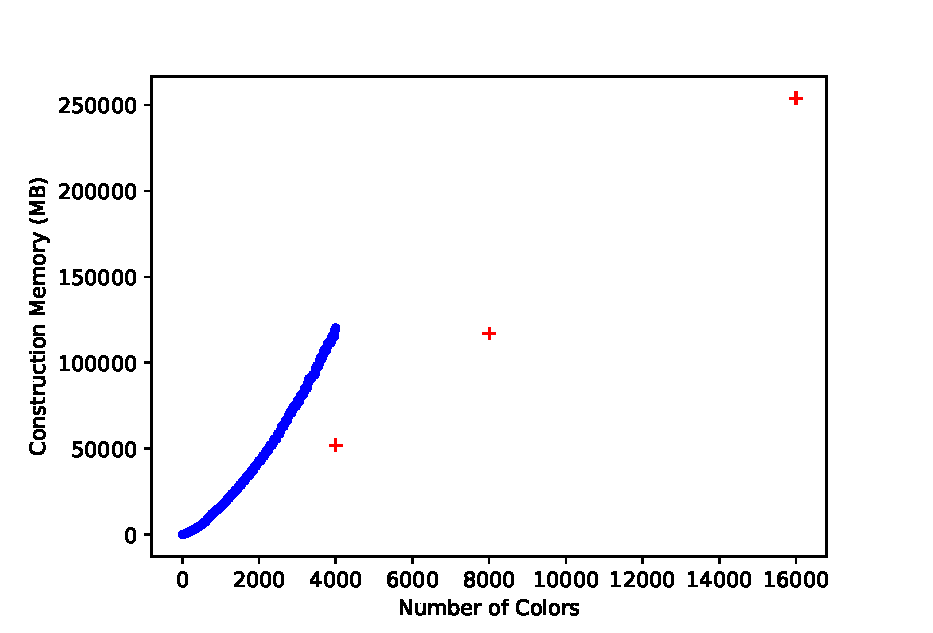
\includegraphics[scale=0.5]{content/BFTvsVARI.eps}
 %\caption{Comparison between Bloom Filter Trie (blue dots) and $\ours$ (red pluses) on isolates from GenomeTrakr.  Bloom Filter Trie was ran on 2,000 isolates and $\ours$ was ran on 4,000.}
 %\label{figure:bftvsvari}
%\end{figure*}


\begin{figure}[h!]
  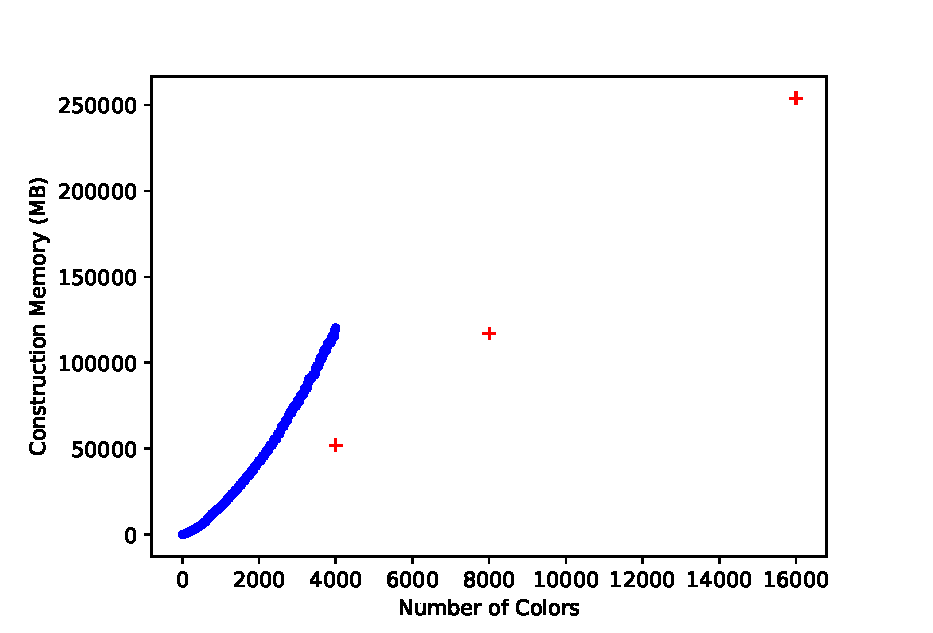
\includegraphics[width=0.55\textwidth]{content/BFTvsVARI.eps}
 \caption{Comparison between Bloom Filter Trie (blue dots) and $\ours$ (red pluses) on isolates from GenomeTrakr.  We ran Bloom Filter Trie on 4,000 isolates and plot $\ours$ results up through 16,000 isolates.}
 \label{figure:bftvsvari}
\end{figure}


\subsection{Comparison to Bloom Filter Trie}

In addition to demonstrating scalability, we used the Samonella strains from GenomeTrakr to directly compare the data structure space and construction memory of $\ours$ with Bloom Filter Trie~\cite{holley2015bloom} (BFT).  We observe both tools have a small memory overhead in construction above the final data structure. We found super-linear growth in BFT construction memory (see Figure \ref{figure:bftvsvari}), and that BFT produced a graph 105 GB in size after 4,000 samples were inserted. This is only slightly less space than the 106 GB the $\vari$ data structure requires to represent twice as many samples.  Holley  et al.~\cite{holley2015bloom} report  sub-linear growth up through 471 samples; however, we posit these differing observations may be a result of both differing dataset and preprocessing methods; More specifically, these isolates were extracted from a single species (humans) in contrast to GenomeTrakr, and thus may result in data that is more more homogeneous and has slower growth in the diversity with population size;  GenomeTrakr Salmonella samples are culled from  diverse food production environments.  Furthermore, they filter $k$-mers that have low multiplicity as a means to clean the data. This may reduce the growth as parts of the so called core genome may be missing in some samples, and the set of population $k$-mers could converge asymptotically toward the core genome.  Though Holley {\it et al.} compared to Sequence Bloom Trees by Solomon {\it et al.}~\cite{solomon2015large}, we do not because the Sequence Bloom Tree software is designed for transcript querying rather than variant detection.  %This may also contribute to different subsets of the true genomes content being considered by tools as datasets grow in size.

%We present Figure \ref{figure:bftvsvari} to illustrate the scalability of $\ours$ and Bloom Filter Trie.

%Preprocessing differences: They take raw reads, k-mer count them (k=63), and discard any k-mers with multiplicity less than 3.  This means k-mers covering read errors will likely be discarded, but might also leave chunks of the genome missing.  As more genomes are added, any 'core genome' components that are missing from individual sets could be found, so under this theory, one would expect the growth to be asymptotic toward capturing the whole 'core genome' in the data structure.  Perhaps this component dominates the growth giving the appearance of sublinear growth.  Under this theory, our assembly preprocessing could be keeping the bulk of the core genome and thus eliminate this component.  Other components of growth that were previously dominated might then become visible.

%Species/environment differences.  They are dealing with a different species and only those samples that can live in humans. So given the narrower environment there may be evolutionary pressure to select just the possible strains that thrive inside a human.  The salmonella in our dataset come from a much wider swath environments, so there is less selective pressure toward a more homogeneous population.  Thus the diversity of the underlying population itself grows faster which is then reflected in memory use.




% 4000 136gb ram, 1tb disk, 9 hours
% 8000 271gb ram, 4.6tb disk, 31hours


% 8000-merge 10gb ram, 6 hours

% 1. merge-2x2 vs vari-4, merge-4x4 vs vari8

% 2. vari, growth experiment with smaller things


% 3. incremental angle

% 4. bloom filter trie

% SO AND SO HAD 100 GENOMES AND ONLY BUILT THE DE BRUIJN GRAPH, but we were more efficient AND we included color too!


\subsection{Validation using E. coli}

%We copied the first $k$ nucleotides from the beginning of the FASTA sequence to the end in order to include $k$-mers lost when the circular genome is linearized to a disk file.

We validate $\ours$ by generating two succinct colored de Bruijn graphs with three \emph{E. coli} assemblies each, merge them, and verify correctness of the merged graph:    First, we generated all $k$-mers for each reference genome, counted all unique $k$-mers with KMC2~\cite{deorowicz2015kmc}, constructed two de Bruijn graphs of three assemblies each using $\vari$, and merged them into a six color graph using $\ours$.  Independently, we constructed a second colored de Bruijn graph using $\vari$ on all six assemblies in one run, and compared these two graphs.  We found $\ours$ produced files on disk that were bit-for-bit identical to those generated by $\vari$, demonstrating they construct equivalent graphs and data structures.

%Second, we partition each reference genome, leading to a de Bruin graph in which some nodes have no successors and others no predecessors.  We recall $\vari$ inserts extra edges for these conditions; however, some extra edges may become obsolete when graphs are merged.  In this situation, we expect the merged graph to have these additional obsolete extra edges relative to a graph built by $\vari$ from the complete set. We verify the equivalence of these graphs by printing the list of edges for the graph merged from two colored de Bruijn graphs (where the number of colors is equal to 3) as well as the colored de Bruijn graph (where the number of colors is equal to 6)  constructed using $\vari$.  We compared the full edge labels and found that the only difference was 126 additional extra edges in the merged graph.  Furthermore, applying VARI's bubble calling method to both graphs returned the same set of bubbles.


 
